%-------------------------------------------------------------------------------
\section{Measurement Methodology}
\label{sec:methodology}
%-------------------------------------------------------------------------------

\begin{figure}[t]
    \centering
    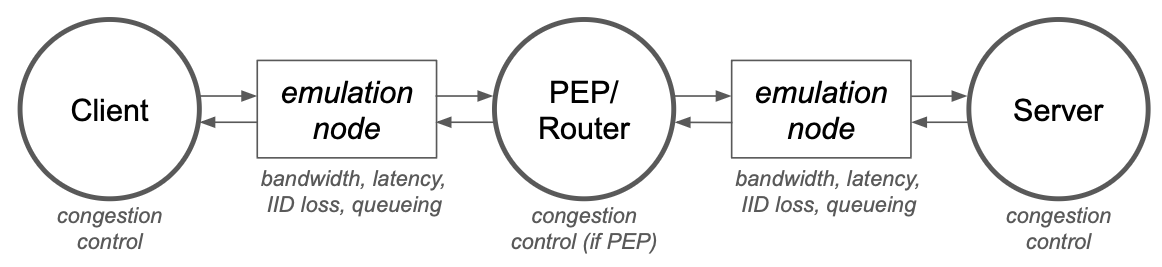
\includegraphics[width=\linewidth]{splitting/figures/mininet-topology.png}
    \caption{Two-segment network topology in \texttt{mininet}. The
     middle node splits the path into two segments with different properties.}
    \label{fig:splitting:mininet}
\end{figure}

\begin{table}[t!]
  \centering
\footnotesize
\begin{tabular}{ l l l l l }
  \toprule
    \textbf{CCA} & \textbf{Implementation}\\
    \midrule
    BBRv3 & Linux TCP v6.4.0+ \texttt{google-bbr/v3} fork\\
    BBRv2 & Linux TCP v6.4.0+ \texttt{google-bbr/v2alpha} fork\\
    BBRv1 & Linux TCP v5.15.0-122-generic \\
    CUBIC & Linux TCP v5.15.0-122-generic \\
    % TCP & BBRv1 & Ubuntu 22.04.2 with Linux kernel 6.1, 6.8; Ubuntu 18.04.1 with Linux kernel\\
    % & & 4.15, 4.16, 4.17, 4.18, 5.0, 5.4, 5.19; Ubuntu 18.04.1 with Linux kernel v4.9,\\
    % & & 4.10, 4.11, 4.12, 4.14 (Docker Ubuntu 16.04 for build)\\
    BBRv3 & Google \texttt{quiche} v131.0.6728.1 \\
    BBRv1 & Google \texttt{quiche} v131.0.6728.1 \\
    CUBIC & Google \texttt{quiche} v131.0.6728.1 \\
    BBRv2 & Cloudflare \texttt{quiche} v0.14 \\
    BBRv1 & Cloudflare \texttt{quiche} v0.14 \\
    CUBIC & Cloudflare \texttt{quiche} v0.14 \\
    BBRv2 & IETF \texttt{picoquic} \texttt{29c7c53} \\
    BBRv1 & IETF \texttt{picoquic} \texttt{29c7c53} \\
    CUBIC & IETF \texttt{picoquic} \texttt{29c7c53} \\
\bottomrule
\end{tabular}
  \caption{\small \label{tab:cca-implementations} The congestion control schemes and
   transport protocol implementations we evaluate in the measurement study.}
  \vspace{-0.4cm}
\end{table}


We want to evaluate different congestion control schemes in a variety of network
settings. To do this, we run emulation experiments in \texttt{mininet} with
simple HTTPS clients and servers to measure the throughputs of long-lived data
transfers. In this section,
we describe our emulated network configurations, HTTPS endpoints and
PEP, and other specifications.

\paragraph{Network configuration.}

We used two linear network topologies: a one-segment topology for caching
end-to-end measurements and a two-segment topology for evaluation with a
connection-splitting PEP (\Cref{fig:mininet}). Both have
a client and server node at each end. The two-segment topology additionally has
a router node in between. Each path segment has a bridging node to emulate network
properties on the link.

We parameterize each path segment in three dimensions: delay, bandwidth, and a
random loss rate. We configure the network properties on the bridging nodes'
egress interfaces, using \texttt{tc-netem} to set delay and random loss,
and \texttt{tc-htb} to set bandwidth. Additionally, we use \texttt{tc-qdisc} to
configure the queues to use RED\footnote{We apply RED and not droptail because it gives more
continuous feedback about loss for congestion control, and is commonly used in
core routers. We also do not need the multi-flow and low-delay properties of
other queue disciplines. We use RED in \texttt{adaptive harddrop} mode with a
maximum queuing delay of $\approx1$ BDP. Exact parameters are available in the code.},
which is the source of congestive loss.
Each link is symmetric in
the uplink and downlink directions. For some versions of BBR, we set an \texttt
{fq} qdisc on the host nodes' egress interfaces for pacing.

\paragraph{Host configuration.}

We create simple HTTPS wrappers around each transport protocol implementation to
evaluate the congestion control schemes in \Cref{tab:cca-implementations}. The TCP
endpoints use the Python \texttt{http} module. For the QUIC implementations, we
modify comparable client/server applications from each repository.
%to transfer some number of bytes from server to client.
With the exception of enabling TCP pacing where required by BBR, we use
``default values'' for tunable parameters, considering these to be part of each
implementation.

In TCP, we set the CCA by using a specific Linux kernel
version and loading the congestion control module. We use the default
kernel's implementations of CUBIC and BBRv1, and Google's kernel fork for
BBRv2 and BBRv3 (\Cref{tab:cca-implementations}).

In QUIC, we simply select the CCA as a command-line
argument to the user space implementation. We evaluate Google \texttt
{quiche}~\cite{google-quiche}, Cloudflare \texttt{quiche}~\cite
{quiche}, and \texttt{picoquic}~\cite{picoquic}. Google and Cloudflare \texttt
{quiche} are their production implementations of the same name,
and \texttt{picoquic} is a minimalist implementation based on the IETF spec.
All three include CUBIC and BBRv1 implementations, as well as some form of
BBRv2 or BBRv3, which is still undergoing standardization.

For the transparent, connection-splitting TCP PEP, we use PEPsal~\cite
{caini2006pepsal}. PEPsal intercepts the SYN packet during the three-way
handshake and forms separate TCP connections with each endpoint,
copying data between the two sockets. Note that
discussions of split QUIC are based only on the split throughput heuristic
and do not use an actual splitter.

\paragraph{Experiment specification.}
In each experiment, the HTTPS client requests a specific number of bytes to be
transferred from the server in the HTTPS payload. This number corresponds to the
amount of data that can be transmitted through the bottleneck link over a
$10$-second period. We have found this to be sufficiently large to reflect
sustained throughput.

In practice, we report the "single-stream goodput" calculated as the number of
application-layer bytes received (excluding HTTPS headers) divided by request
completion time (from when the client sends a request to when it receives a
complete response). Due to header overhead and request latency, this metric
will never equal the link rate.
% \thea{could add, may not be necessary: A more precise measurement would use the
%  same application for each CCA and invoke lower-level APIs, but with large data
%  transfers, minor differences in client/server implementations will not impact
%  observed trends. }
% \thea{say something about how long the flow is? + why this is limited but still
%  useful}.

\paragraph{Machine specification.} All experiments use CloudLab~\cite
 {duplyakin2019design} x86\_64 rs630 nodes in the Massachusetts cluster running
 Ubuntu 22.04.2. The nodes use the default Linux kernel v5.15.0-122-generic,
 except for TCP BBRv2 and BBRv3.%, in which they use the Google fork of v6.4.0+.
